\chapter{Understanding Electrical Data}
As machine learning techniques have become the de facto approaches for Big Data analytics, these techniques are also applied and adapted to process and analyze electrical data. A common objective of the electrical data analysis is to recognize and identify patterns, or signatures of events that occur on the Smart Grid. Therefore, a large number of these approaches are based on pattern recognition \cite{al2012synchrophasor}.Finding pattern or recognizing pattern can be considered as fitting a model in the data. Such an outcome is the result of a cascaded work process namely preparing data, searching pattern, evaluating knowledge and finally referring it towards the monitoring and control units. We look at each of this briefly to understand the data thoroughly before diving into anomaly detection methods. We visualize our data, looking for inital ideas in determining patterns of electrical data using state of art machine learning libraries. 

Data preparation includes data cleaning, data integration and transformation, data reduction and data warehousing which will explained in detail below. Before diving deep into understanding the data process-by-process, what we might learn from the dataset includes:

\begin{itemize}

  \item The number of records in the dataset
  \item The number of attributes (or features)
  \item For each attribute, what are the datatypes(nominal, ordinal, or continuous)
  \item For nominal attributes, what are the values
  \item For continuous attributes, the statistics and distribution
  \item For any attributes, are there any missing values
  \item For any attributes, the number of distinct values

\end{itemize}

\begin{enumerate}
\item\textbf{Preparing Data:} Machine learning algorithms learn from data. It is critical that we feed them the right data for the problem we want to solve \cite{brownlee2013prepare}. Even if we have good data, we need to make sure that it is in a useful scale, format and even that meaningful features are included. This data preparation process has direct impact on the result, the more discipline we are in handling the data, the more consistent and better result we will able to achieve. Below are the three important data processing steps widely followed when using machine learning algorithms, namely:
	\begin{enumerate}
		\item\textbf{Selection of Data:} Our dataset is a collection of huge volumes of electrical distribution measurements. Identifying patterns by running through all this data is time consuming, so we consider subsets of it for our analysis. The subsets are carefully chosen so that we may not miss out important information related to identifying anomalies. The data obtained is measured by sensors deployed across the distribution network and this data is available for the wholeday read around every second. Hence we have 24*60*60 = 86400 observations for a complete day, so by taking one or two weeks of data in the form of two different sets (weekday data of normal working days and weekends data following the normal working days) without any holidays from a particular region would be good and big enough to be assured of not missing any relevant information. 
		\item\textbf{Preprocessing Data:} We now have selected data which needs to be preprocessed before we can apply anomaly detection methods. The performance of anomaly detection methods depends vastly on how clean the data is, do we need to format the data and is there any noise data in it. Cleaning the data is removal of redundant values which we can see by looking at the data or by fixing the missing data. In our electrical data, we have values such as energy transported and energy consumed which contain previous day values along with currently measured value which is not necessary for anomaly detection. Likewise we have reactive current values which are available for few regions and not available in few, therefore we can remove these missing and non-important data. In order to remove the noise we can use data smoothing techniques which will be discussed later.
		\item\textbf{Transformation of Data:} We have selected the dataset which is big enough, cleaned and formatted the data which looks good for analysis but, in order for the machine learning algorithms to fit the data to the proposed model we need to transform the data accordingly. One method which plays very important role for our anomaly detection process is scaling. We have mixture of values in our dataset like, voltages, current, power, phase displacement which are measured on different scales( volts, amperes, watts, degree) and hence bringing these values under one common scale can prove beneficial for our detection process. Principal Component Analysis(PCA) is yet another technique which transforms the data such that the data are represented according to the variances. Its a very useful statistical method widely used in machine learning for reducing the dimensions of the data. We have even proposed the detection of anomaly method using PCA in our work which will be discussed in detail later. Likewise we can also use data decomposition and aggregation when necessary. 
	\end{enumerate}



\item\textbf{Searching Patterns in the data:} Our next step in understanding the data is finding about the patterns in the data. Several statistical methods are already readily available which we will leverage for working with our electrical data. Some of the methods which we believe would be an asset in finding the patterns in our electrical data are briefly discussed below:
\begin{enumerate}
\item\textbf{Correlation:} Correlation is a statistical technique which tells you how variables in our dataset are related. A simple correlation plotted against our set of electrical data is as shown in the Fig \ref{fig:correlation}. We have used the existing correlation method available under python pandas library. It computes the \textit{pearson} correlation coefficient which is the default correlation method available along with \textit{kendall} and \textit{spearman}. The details of these methods are not covered here, as it is out of scope of our work. The correlation measure as in the figure provides us with initial information about which features to consider and which features will not be so useful in finding the patterns. The correlation matrix is calculated across each column of our dataset. Some important observations are, variables which are directly related have high correlation values meaning, an increase in the value of one variable increases the corresponding related variable and similarly a low correlation value means the two columns are independent of each other. 

\begin{figure}[tph!]
\centerline{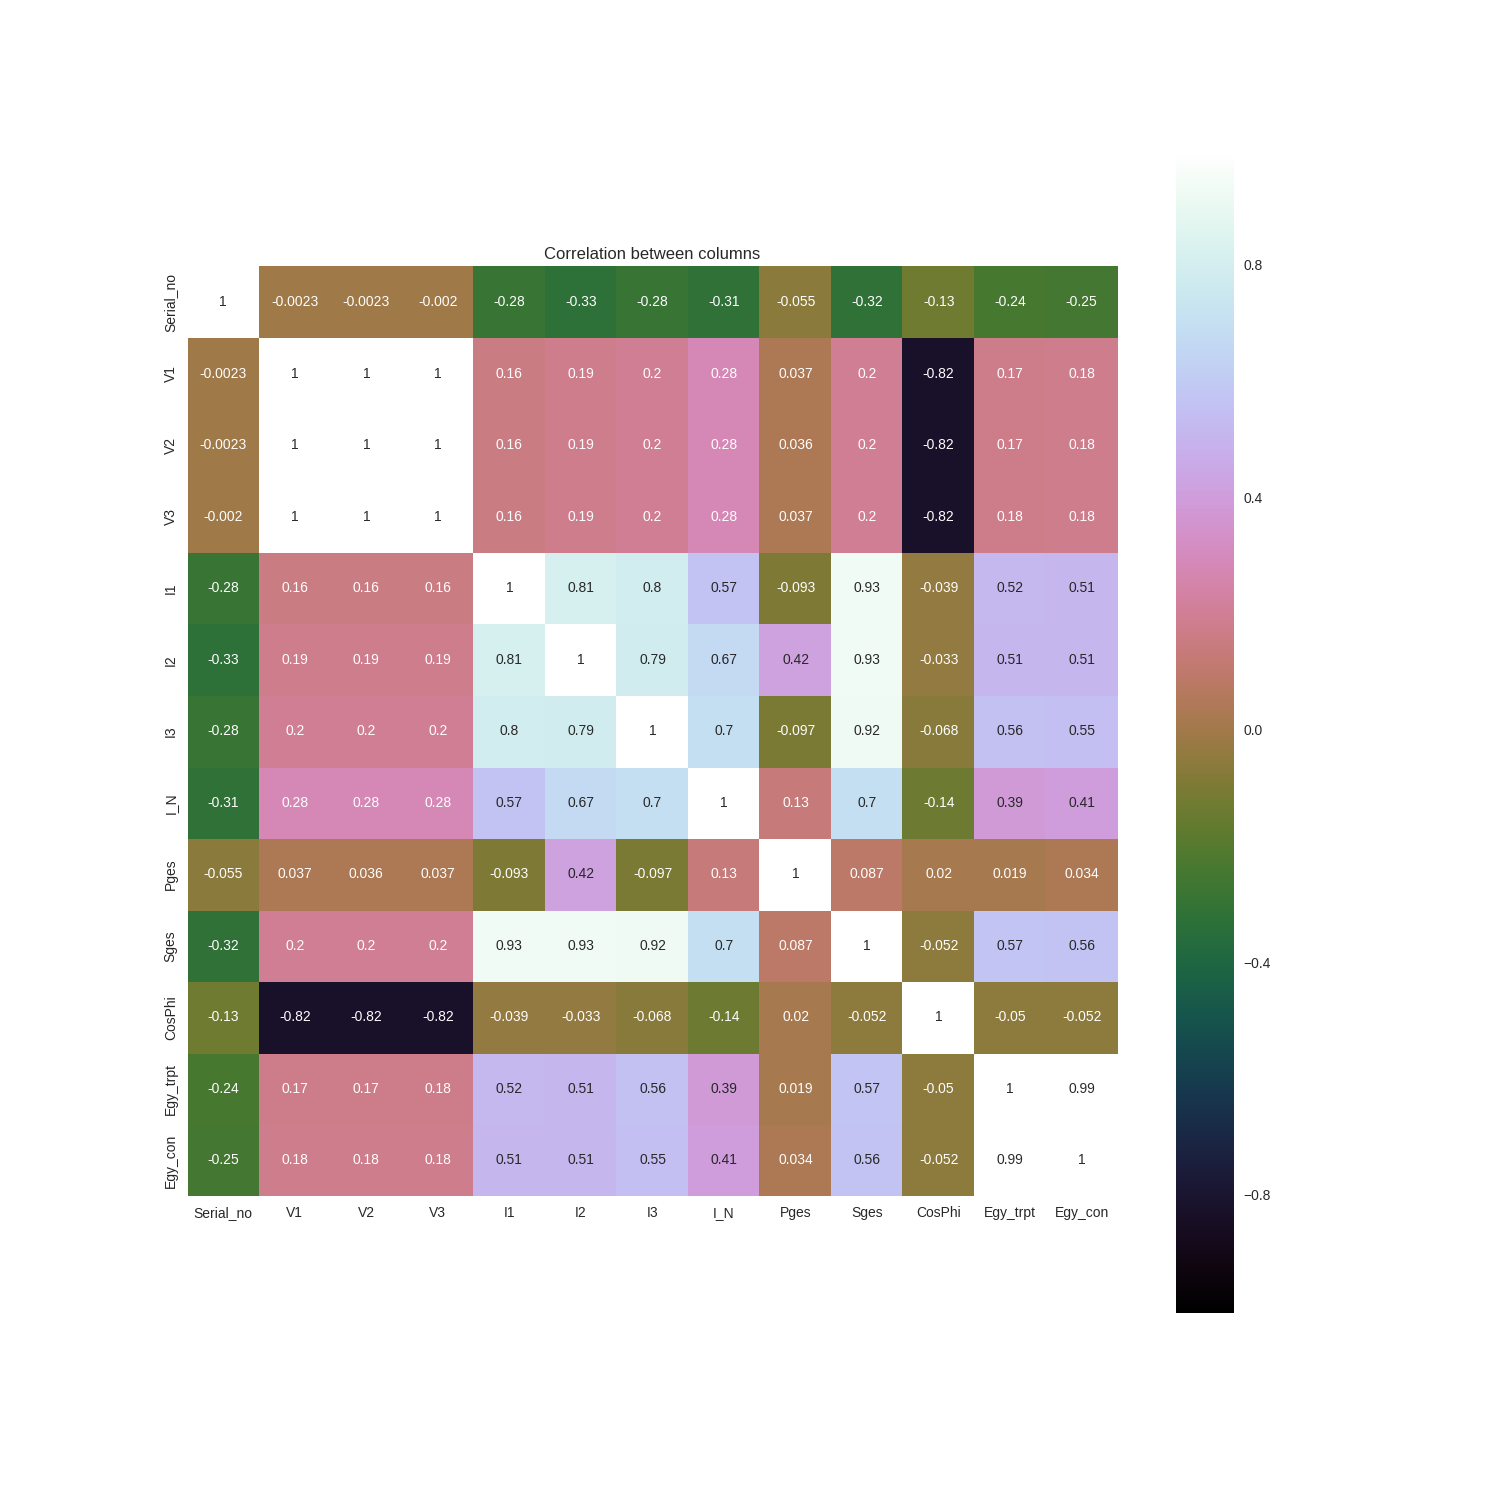
\includegraphics[totalheight=10cm]{Correlation.png}}
\caption{Correlation matrix of Data}
\label{fig:correlation}
\end{figure}
A positive correlation indicates the two columns behave similar that is, for two positively correlated variables 'a' and 'b', the value of 'b' increases with increase in 'a' and correspondingly decreases with decrease in 'a'. A negative correlation is vice versa, increase in value of 'a' decreases 'b' and decrease in value of 'a' increases the value in 'b'.  A correlation value of 1 and closer to 1 are said to be highly correlated, as you can see the diagonal elements in the figure all have values 1 which means the column values are highly correlated among themselves, while the column variables representing voltages seem to have very less correlation with current and power consumed/transported  values. Such less correlated values can be considered as potential columns for our analysis in finding the anomalies as these values are independent of each other. We concentrate on these low correlated columns and believe highly correlated values are not so important for our research.

\item\textbf{Histogram:} Histograms are another way of visualizing the data to get the initial look of how our data is distributed. For continuous variables as in our case, a histogram can be used to assess the spread and shape of our data and suits particularly well when we have large number of observations. Bins in the histograms define the width of the class intervals, with sufficient number of bins, histograms will provide the peak and unusual data details. A simple histogram plot for our dataset which has been normalized to mean=0 and variance=1 is as shown in the Fig \ref{fig:hist1}. We can see that the data is following a normal distribution with the tails distributed on either side of mean and in between -5 and +5. We can also deduce from the Fig \ref{fig:hist1} that the data points are likely to occur mostly near the mean and the occurence of points decreases on both sides of mean and becomes more less probable. This means that a value which tends to move very much further away from the mean will be less probable and can be considered as outlier in our distribution. 
\begin{figure}[tph!]
\centerline{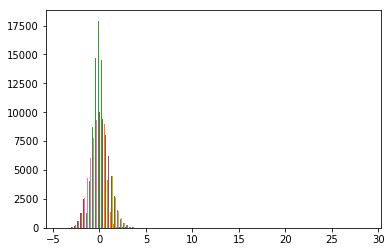
\includegraphics[totalheight=6cm]{histogram.png}}
\caption{Histogram of the data}
\label{fig:hist1}
\end{figure}
\item\textbf{Box and whisker plot:} Till now we have considered techniques which make use of the entire columns. Let us look at single column and check how the values in each column look like. We can get to know what is the maximum, minimum and mean value of each column by using box and whisker plots. The plot displays some important information for instance, the range, median and quartile, which reflects the actual data. It is yet another technique used in exploratory data analysis, a numerical detective work which uncovers the possibility of quantitative interrelationships among the data \cite{larsen1985box}. The box and whisker plot of first 100 values of Voltage V1 is as shown in the Fig \ref{fig:boxplot}. Among the 100 values, the topmost point in the figure shows the maximum value, the bottommost point shows the minimum value. The topmost and the bottommost points are called whiskers, the rectangle has the lower and upper quartile constituting inter-quartile range and the median is represented by the orange line inside the rectangle. This gives us the idea of how the column values are distributed numerically. The points  which lies outside 3 times of interquartile range can be suspected to be an outlier or an anomaly point.
\begin{figure}[tph!]
\centerline{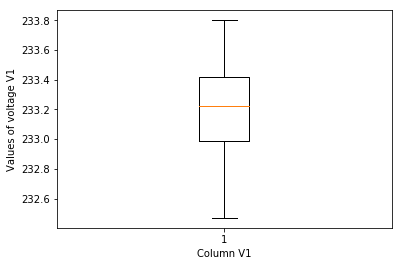
\includegraphics[totalheight=6cm]{Boxplot.png}}
    \caption{Box plot of first 100 values of Voltage V1 }
    \label{fig:boxplot}
\end{figure}
\item\textbf{GGplot:} Another useful visualization tool for identifying relationship between column values in our data is ggplot. GGplot does this by mapping the values of two columns against each other. We can view this as an alternative approach to correlation but, with the distribution of points. Correlation matrix will give you the measure of how two column values are related by a numerical value between 0 and 1, while ggplot will help you visualize the column values individually in the form of scatter plot and aid the process of understanding the electrical data in much easier way. We have plotted voltage value V1 against the phase displacement value CosPhi in the Fig \ref{fig:ggplot}. We can make a conclusion that most of the values of voltages are within the range of 225 and 240 volts, whereas the CosPhi values are within the range of 0.75 to 1. The values very far from this range can be considered as unusual.
\begin{figure}[tph!]
\centerline{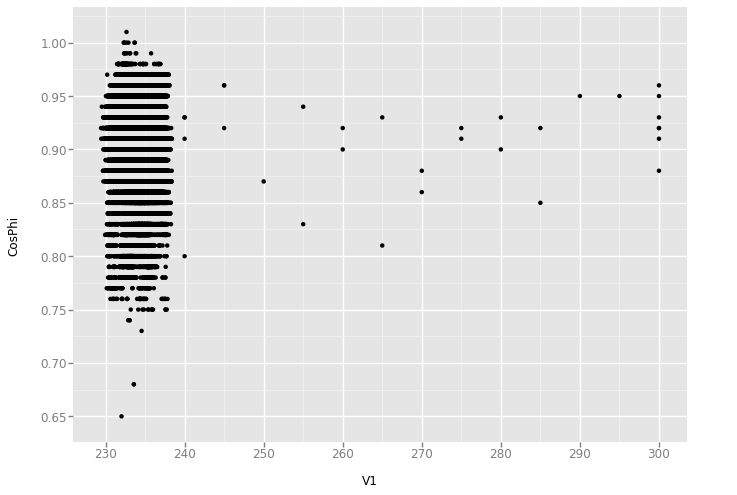
\includegraphics[totalheight=6cm]{ggplot_V1_CosPhi.png}}
\caption{ggplot of Voltage versus Phase Displacement.}
\label{fig:ggplot}
\end{figure}
\end{enumerate}
				
	
\item\textbf{Knowledge Discovery:}




\item\textbf{Evaluating against the goal:}
\end{enumerate}
In order to visualize the huge set of electrical data collected from electrical grids we had to store all the data in a database. Storing the data into the database will not only allow us to compute the statistics better but also, will enable us to clearly visualize the patterns of the data in time windows such as weekday patterns, weekend patterns, hourly patterns and so on.  Below we will discuss the structure of the data stored in the database: \\
\subsubsection*{Tablename:    Energy-Data} 
\begin{center}
    \begin{tabular}{ | l | l | l | l | l |}
    \hline
    \textbf{Column Name} & \textbf{Data Type} & \textbf{Default Value} & \textbf{Characteristics} & \textbf{Key} \\ \hline
    Serial No & int & NOT NULL & AUTO-INCREMENT & Primary Key\\ \hline
    Date & DATE & NOT NULL &  & \\ \hline
    Time & TIME & NOT NULL & & \\ \hline
    V1 & DOUBLE & NULL & & \\ \hline
    V2 & DOUBLE & NULL & & \\ \hline
    V3 & DOUBLE & NULL & & \\ \hline
    I1 & DOUBLE & NULL & & \\ \hline
    I2 & DOUBLE & NULL & & \\ \hline
    I3 & DOUBLE & NULL & & \\ \hline    
    I-N & DOUBLE & NULL & & \\ \hline
    Pges & DOUBLE & NULL & & \\ \hline
    Sges & DOUBLE & NULL & & \\ \hline
    CosPhi & DOUBLE & NULL & & \\ \hline
    Egy-trpt & DOUBLE & NULL & & \\ \hline
    Egy-con & DOUBLE & NULL & & \\ \hline
    Location & VARCHAR(50) & NOT NULL & & \\
    \hline
    \end{tabular}
\end{center}

\subsubsection*{Data Description:}
 \begin{enumerate}
\item \textbf{Serial No}: This is the primary key to uniquely identify the record. This field will contain the serial numbers of the record. By record, while considering databases, we mean a row in the table Energy-Data.
\item \textbf{Date}: This field contains the date of the data. The value is stored in date format( 'YYYY-MM-DD').
\item \textbf{Time}: This field specifies the time when the data was collected. This value is stored as (hh:mm:ss).
\item \textbf{V1}: This is the voltage-1 of the 3-phase voltage expressed in Volts(V) which is stored as a double data type. 
\item \textbf{V2}: This is the voltage-2 of the 3-phase voltage expressed in Volts(V) which is stored as a double data type.  
\item \textbf{V3}: This is the voltage-3 of the 3-phase voltage expressed in Volts(V) which is stored as a double data type. 
\item \textbf{I1}: This is the current in Phase-1 of the 3-Phase current expressed in Amperes(A)which is stored as a double data type. 
\item \textbf{I2}: This is the current in Phase-2 of the 3-Phase current expressed in Amperes(A) which is stored as a double data type. 
\item \textbf{I3}: This is the current in Phase-3 of the 3-Phase current expressed in Amperes(A) which is stored as a double data type. 
\item \textbf{I-N}: This is the neutral current passing through the network which will be accounted for calculation of reactive power which is stored as a double data type. 
\item \textbf{Pges}: Real power of the network, also known as working power expressed in units of Watts(W). It is stored as double datatype. Its the product of Sges and CosPhi values.
\item \textbf{Sges}: Actual power of the network, also known as apparent power calculated as a product of Voltage and Amperes expressed as Voltage-Ampere(VA). It is stored as double data type.
\item \textbf{CosPhi}: Power displacement, also known as phase displacement in the network. Sometimes referred to as Power factor which has no units, stored as double datatype.
\item \textbf{Egy-trpt}: Energy tranported in the network expressed in terms of Wattage-hour(Wh). Stored as double value.
\item \textbf{Egy-con}:  Energy consumed at the receiver end as calculated by the smart meters. Expressed in terms of Wattage-hour(Wh), also stored as double datatype.
\item \textbf{Location}: New field added to the database which is not available in the csv files collected from the electrical grids. This field will be able to identify the data region which is very helpful for data analysis. Stored as string in the database.
\end{enumerate}
\label{sec:Understanding Electrical Data}